\documentclass{article}
\usepackage{graphicx}
\usepackage{float}
\usepackage[spanish]{babel}
\usepackage{hyperref}
\usepackage{csquotes}
\graphicspath{ {img/} }
\setlength{\parskip}{\baselineskip}

\title{Compila la UI de una APP \\[3ex] \small PAMN - Programación de Aplicaciónes Moviles Nativas}

\author{Chamil José Cruz Razeq}

\begin{document}
    \maketitle
    \thispagestyle{empty}
    \newpage

    \section{Introducción}
        Todos los informes sobre las tareas propuestas se encuentran disponibles en el
         siguiente repositorio de \href{https://github.com/chamilstudy/ulpgc_pamn_assigments}{GitHub}.

        Por otro lado las resoluciones se contrarán en sus respectivos repositorios
        \href{https://github.com/chamilstudy/ulpgc_pamn_codelab3.1}{Codelab3.1} y
        \href{https://github.com/chamilstudy/ulpgc_pamn_codelab3.2}{Codelab3.2}.

    \section{Codelab 3.1: Aplicación de Tiradas de Dado}

    Se ha desarrollado un programa de lanzamiento de dados utilizando los recursos
     facilitados el curso \cite{codelab}. Dentro de las características desarrolladas
     destaca la actualización de la imagen del dado respecto al valor randomizado obtenido
     al presionar el botón [ Figura \ref{fig:dice} ]. Además te hace enfasis en el uso del 
     fichero "strings".
    
     \begin{figure}[H]
        \centerline{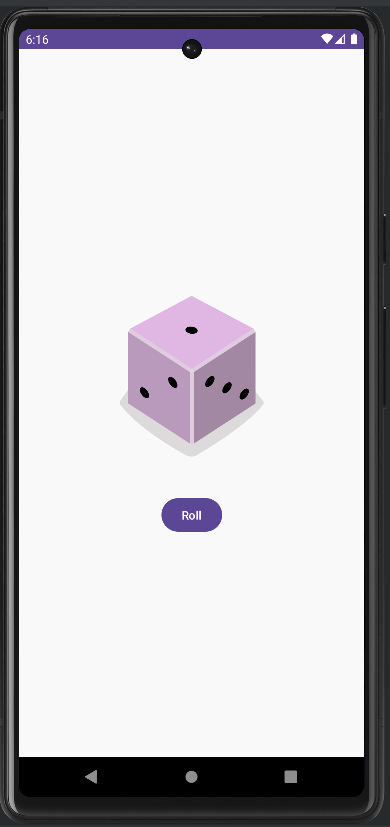
\includegraphics[scale=0.3]{dice.png}}
        \caption{Aplicación de lanzamiento de dados}
        \label{fig:dice}
    \end{figure}

    Adicionalmente, el curso propone el uso del debugger para familiarizarse con el
     entorno de desarrollo.

    \section{Codelab 3.2: Aplicación de Limonada}

    Para el desarrollo de esta aplicación se ha tenido en consideración lo aprendido en el
     ejercicio de lanzamiento de dados. Conservando las prácticas anteriores se ha hecho uso
     del fichero "strings" para localizar las descripciones de las imagenes y frases.

    La aplicación consiste en crear un proceso de elaboración y consumo de limonada, donde
     se cargará y actualizará una imagen, su descripción y la frase con cada click sobre la misma. Adicionalmente, se 
     ha programado el paso 2 [ Figura \ref{step2} ] (relativo a exprimir un limón) de tal manera que no se continuará
     hasta el siguiente paso hasta que se haya presionado la imagen un máximo (aleatorio) de veces.

     \begin{figure}[H]
        \centerline{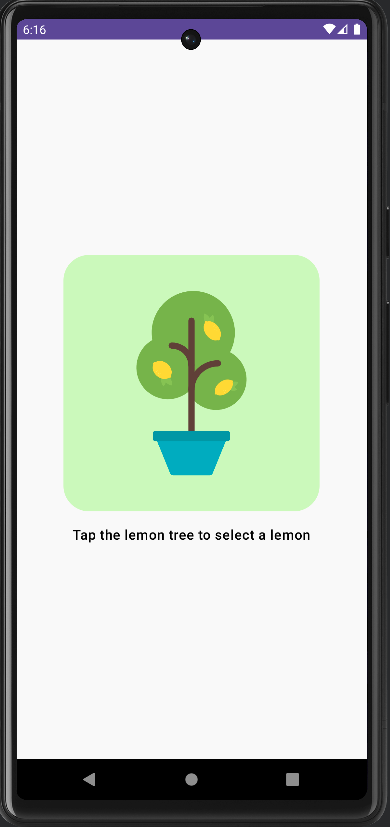
\includegraphics[scale=0.2]{step1.png}}
        \caption{Paso 1 de la aplicación de limonada}
        \label{fig:step1}
    \end{figure}
    \begin{figure}[H]
        \centerline{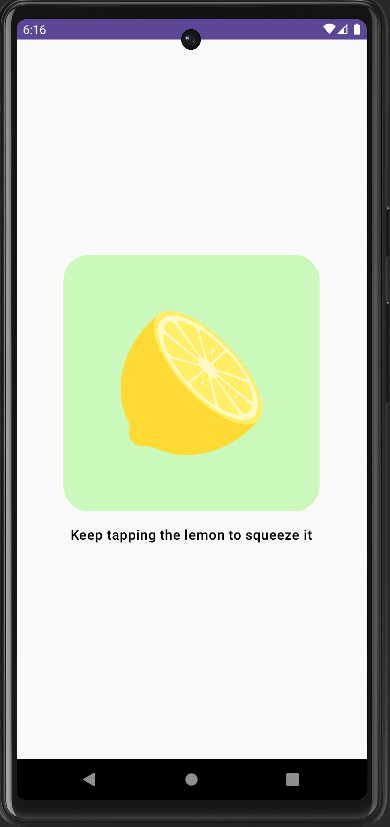
\includegraphics[scale=0.2]{step2.png}}
        \caption{Paso 2 de la aplicación de limonada}
        \label{fig:step2}
    \end{figure}
    \begin{figure}[H]
        \centerline{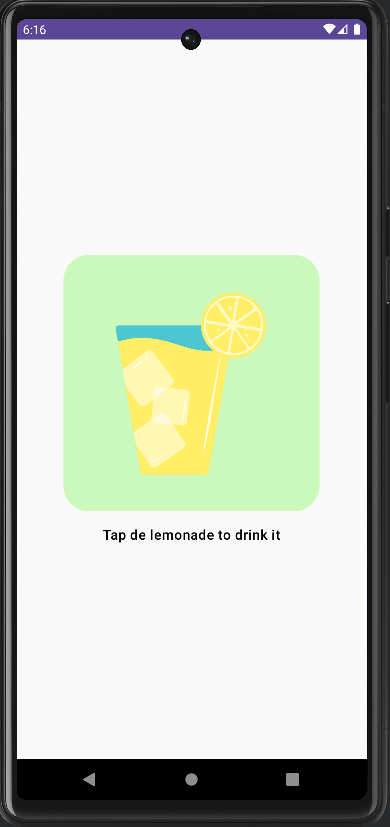
\includegraphics[scale=0.2]{step3.png}}
        \caption{Paso 3 de la aplicación de limonada}
        \label{fig:step3}
    \end{figure}
    \begin{figure}[H]
        \centerline{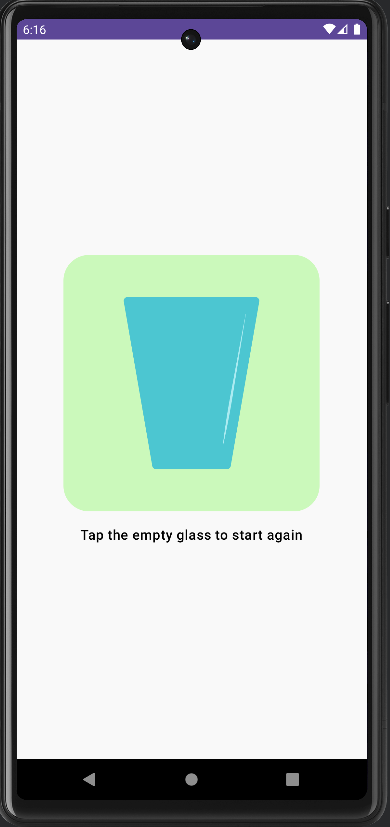
\includegraphics[scale=0.2]{step4.png}}
        \caption{Paso 4 de la apliación de limonada}
        \label{fig:step4}
    \end{figure}

    \begin{thebibliography}{}
        \bibitem{codelab} Codelab Compila la IU de una APP - https://developer.android.com/courses/android-basics-compose/unit-2?hl=es-419
    \end{thebibliography}
        
\end{document}